% !TEX program = pdflatex
% !TEX encoding = UTF-8
% !TEX spellcheck = en_US

\documentclass[11pt, a4paper, notitlepage]{article}

\usepackage{settings}

\geometry{margin=1cm}
\graphicspath{./}
\addbibresource[label=main]{./publications.bib}


%---------------------------------------------------------------------------------------------------------------------------------------------
%				DOCUMENT
%---------------------------------------------------------------------------------------------------------------------------------------------
\begin{document}
\fontencoding{T1}\selectfont
\pagestyle{empty}
% -------------------------------------- FRENCH VERSION ------------------------------------------------
	\newpage
	\selectlanguage{french}
	
	\cvname{Milan Skocic, PhD}
	
	\cvjob{Electrochimie et Matériaux}
	
	\cvinfo{milan.skocic@gmail.com}
	{+33(0)6 66 18 69}
	{github.com/MilanSkocic}
	{19 avenue Nicéphore Niepce, 71100 Chalon-Sur-Saône, France}
	{0000-0003-2189-5766}


	%----------------------------------------------------------------------------
	\section*{Activités professionnelles}
	\cventry{Mai 2017}{Aujourd’hui}{PhD, Electrochimiste}{Framatome}{France}
	\begin{jobdetails}		
		\item Gestion de projet
		\item Electrochimie à haute température
		\item Corrosion des alliages de Zr et de Ni en milieu aqueux à haute température
	\end{jobdetails}

	\cventry{Oct. 2015}{Fév. 2017}{PhD, Matériaux Métalliques}{Areva NP}{}
	\begin{jobdetails}
		\item Gestion de projet
		\item Corrosion sous contrainte de l’Inconel 718 : traction lente à HT/HP
		\item Corrosion des alliages de Zr : électrochimie à HT/HP
	\end{jobdetails}

	\cventry{Oct. 2012}{Oct. 2015}{Thèse CIFRE - "Etude photoélectrochimique de la Shadow Corrosion"}{Areva/SIMaP Lab.}{France}
        \begin{jobdetails}	
		\item Conception et réalisation d’une cellule électrochimique pour des tests de corrosion a` HT/HP
		\item Validation de la cellule électrochimique à HT/HP
		\item Caractérisations (photo-)électrochimiques à HT/HP
		\item Tests classiques de corrosion en autoclave à HT/HP
		\item Couplage avec une boucle de contrôle de la chimie
	\end{jobdetails}
	
	\cventry{Fév. 2012}{Aout. 2012}{PFE - "Plaques bipolaires métalliques pour PEMFC"}{Air Liquide}{France}
	\begin{jobdetails}
		\item Etude bibliographique sur les aciers inox revêtus
		\item Mise en place des tests de corrosion
		\item Mesure de résistance de contact et observations MET/MEB
		\item Interface avec les différents partners du projet
	\end{jobdetails}

	\cventry{Avr. 2011}{Aout. 2011}{Assistant ingénieur – "Aciers à composition graduée"}{McMaster University, Materials Engineering Department}{Canada}
	\begin{jobdetails}
 		\item Cémentation
 		\item Préparation et caractérisation des échantillons (fraction de phase)
 		\item Modélisation des contraintes maximales en compression
	\end{jobdetails}

	\cventry{2007}{2009}{ArcelorMittal R\&D center}{France}{Technicien}
	\begin{jobdetails}
  		\item Préparation des échantillons : découpe, enrobage, polissage
  		\item Caractérisation microstructurale : MEG-FEG, MET, diffractomètre RX
  		\item Traitements thermomécaniques : Gleeble, laminage à chaud (pilote), machine de traction
	\end{jobdetails}

	\cventry{Août. 2005}{Juin. 2006}{Technicien}{Centre de Pyrolyse (CPM)}{France}
	\begin{jobdetails}
  		\item Réalisation de test de pyrolyse en four pilote
		\item Préparation et caractérisation des échantillons de charbon et de coke
	\end{jobdetails}
	
	\newpage
	
    %---------------------------------------------------------------------------------------------
	\section*{Formations}
	\cvedentry{2012}{2015}{PhD, Materiaux et Electrochimie}{Université de Grenoble}{France}

	\cvedentry{2012}{2015}{Ingénieur, Electrochimie}{Grenoble INP (PHELMA)}{France}
	
	\cvedentry{2003}{2005}{Technicien, Chimie Analytique}{Université de Metz}{France}

	%----------------------------------------------------------------------------------------------
	\section*{Langues}
	Serbe \faStar\faStar\faStar\faStar\faStar \hfill
    Français \faStar\faStar\faStar\faStar\faStar \hfill
    Anglais \faStar\faStar\faStar\faStar\faStarO
	
	%----------------------------------------------------------------------------------------------
	\section*{Compétences en informatique}
	\begin{center}
	    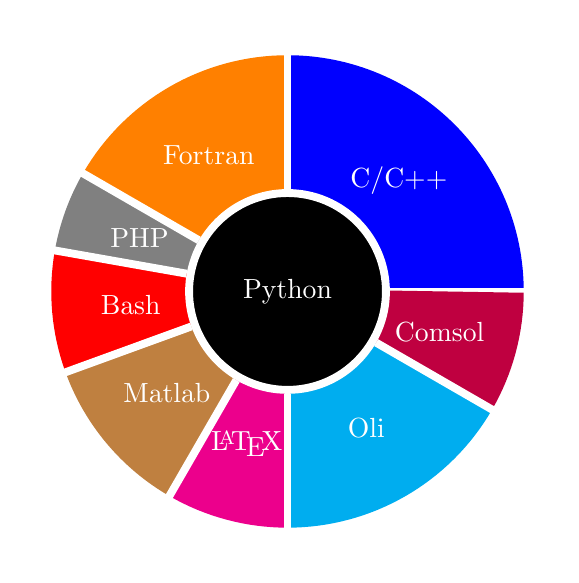
\begin{tikzpicture}[text=white, border/.style={line width=20mm}]
		\foreach \angle/\col [remember=\angle as \last (initially 0)] 
		    in {90/blue, 150/orange, 170/gray, 200/red, 240/brown, 270/magenta, 330/cyan, 360/purple}{
			\draw[\col, border] (\last:2cm) arc[start angle=\last, end angle=\angle, radius=2cm];
			\draw[white, line width=1mm] (\last:1.3)--++(\last:2.0);}
			\node[line width=1mm, draw, circle, minimum width=2.5cm, white, fill=black]{Python};
			\node at (45:2cm) {C/C++};
			\node at (120:2cm) {Fortran};
			\node at (160:2cm) {PHP};
			\node at (185:2cm) {Bash};
			\node at (220:2cm) {Matlab};
			\node at (255:2cm) {\LaTeX};
			\node at (300:2cm) {Oli};
			\node at (345:2cm) {Comsol};

	    \end{tikzpicture}
	    \end{center}
	
    %----------------------------------------------------------------------------------------------
    \section*{PhDs - Support technique}

    \href{https://tel.archives-ouvertes.fr/tel-02304680/}{S. El Euch, “Recherche d’une corrélation entre caractéristiques électrochimiques et relâchement en nickel de l’alliage 690 en milieu primaire d’un réacteur à eau pressurisée,” Université Sorbonne, Paris, 2019.}
 	
    \href{http://www.theses.fr/s222058}{F. Da Fonseca, “Etude du phénomène de shadow corrosion des alliages de zirconium dans les réacteurs à eau bouillante (REB),” Université de Grenoble Alpes, Grenoble, 2021.}


    \href{http://www.theses.fr/s217506}{J. Ben Mohamed, “Etude des mécanismes de Corrosion sous contrainte des alliages 600/690 en milieu secondaire des réacteurs REP en présence de plomb et de soufre.,” Ecole Nationale Supérieure des Mines de Saint-Etienne, Saint-Etienne, 2021.}
    
    \href{http://www.theses.fr/s278984}{D. Peyret, “Mécanismes électrochimiques de la corrosion des alliages de type ZrNbX en condition simulées de réacteur à eau pressurisée,” Université Sorbonne, Paris, 2023.}
	
    %----------------------------------------------------------------------------------------------
	\newpage
	\nocite{*}
	\printbibliography[title=Publications]
	
\end{document}
